\documentclass{article}
\usepackage{tikz}
\author{Asher Griess, David Medin}
\title{R Tree Algorithm}
\begin{document}
\maketitle

\section{Abstract}
An R Tree is a data structure used to make spacial computation and comparison much faster than brute force.  ...

\section{Use Cases}
The R-tree is very similar to the B-tree in structure, and Quad-Tree in use. One of the main differences is that
R-trees are pageable. This means that they could be put into storage, which could be ideal for very large data sets
that can't be stored in ram. You can also take out parts of the R-tree into ram while working with it. A good example
of a program that could use R-trees is a mapping system of the world, where the large data set would be hard to store in memory.
The R-tree is also very good for nearest neighbor searching. Also R-tree can be used to store any type of shape which allow for shapes
of things such as buildings to be put in the minimum bouding rectangle. R-trees have also been used a lot in databases for spacial data.


\section{Inserting}
Complexity

average : none

worst case : $O(n)$

When splitting we are trying to find the best leaf node
that will have least increase to the minimum bounding rectangle.
It should also be noted that when we are at M leafs at every node we are going
to need to perform a split where M is the max children per node.

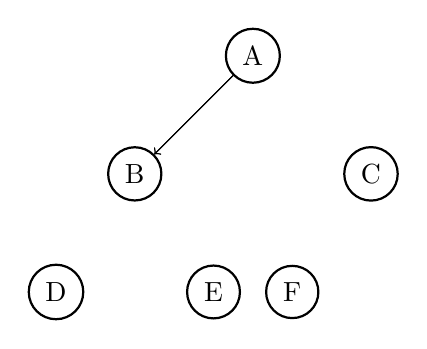
\begin{tikzpicture}
\begin{scope}[every node/.style={circle,thick,draw}]
    \node (A) at (2.5,4) {A};
    \node (B) at (1,2.5) {B};
    \node (C) at (4,2.5) {C};
    \node (D) at (0,1) {D};
    \node (E) at (2,1) {E};
    \node (F) at (3,1) {F} ;
    
\end{scope}

begin{scope}[>={Stealth[black]},
              every edge/.style={draw=black,very thick}]
              \path [->] (A) edge (B);
              \path [->] (A) edge (B);
\end{tikzpicture}
\section{Splitting} 

\section{Searching}
Complexity
Average : $O(log_Mn)$
Worst Case : $O(n)$

\section{Removing}

\section{Citation}

% \subsection*{Part One point one}
% uhhhuhhu huhu.
% text \textbf{bold text} text. Some math: $2+2=5$

% \begin{tikzpicture}[main/.style = {draw, circle}]
% \node[main](1){$x_1$};
% \end{tikzpicture}

\end{document}